In der Datenanalyse soll nun ein Vergleich der interpolierten Daten aus der Wetterstation mit den Wetterdaten des metereologischen Instituts der LMU angestellt werden. Hierbei kann auch die Implementierung der Sonnenauf- und Sonnenuntergangsadaption veranschaulicht werden. Dabei soll der Root Mean Square Error die Prognosegüte der meisten interpolierten Daten veranschaulichen. Die Berechnung erfolgt dabei wie folgt \cite{Armstrong.1992}.
\begin{gather} 
RMSE = \sqrt[2]{\frac{\sum_{t=s}^{S}(Y_{LMU_{t}}-Y_{HKW_{t}})^2}{S}}\\
\begin{matrix} 
   \text{mit:} &&\\ 
   S & \text{--} & \text{Anzahl der Messpunkte innerhalb eines Tages,} \\ 
   s & \text{--} & \text{Prognosezeitpunkt,} \\
   Y_{HKW_{t}} & \text{--} & \text{HKW Wetterdaten zum Prognosezeitpunkt t,} \\ 
   Y_{LMU_{t}} & \text{--} & \text{LMU Wetterdaten zum Messzeitpunkt t.} \\ 
\end{matrix}\notag 
\end{gather} 
%Sonnenscheindaueranfang
\section{Sonnenscheindauer}
\begin{wrapfigure}[13]{l}{0.4\textwidth}
\centering
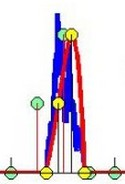
\includegraphics{analyse/sunriseadaption}
\caption{Ergebnis der Sonnenaufgangs- und Untergangsadaption}
\label{fig:sunriseadapt}
\end{wrapfigure}
An dieser Stelle soll zunächst das Ergebnis der Sonnenauf- und Untergangsadaption gezeigt werden. Wie in der Abbildung \ref{sunriseadapt} zu erkennen, würde ohne diese Adaption die Spline Kurve durch die grünlich markierten Punkte verlaufen. Wobei der erste und letzte Punkt, den Tagesbeginn bzw. das Tagesende markieren. Das hieße aber, dass es Globalstrahlung den ganzen Tag über geben würde. Die von der Wetterstation gelieferten Werte müssen daher auf den Zeitraum von Sonnenaufgang- bis Sonnenuntergang, hier als gelbe Punkte auf der x-Achse dargestellt, gemappt werden. Das Mapping der Werte geschieht dabei in gleichen Abständen.
\begin{figure}[htbp]
\centering
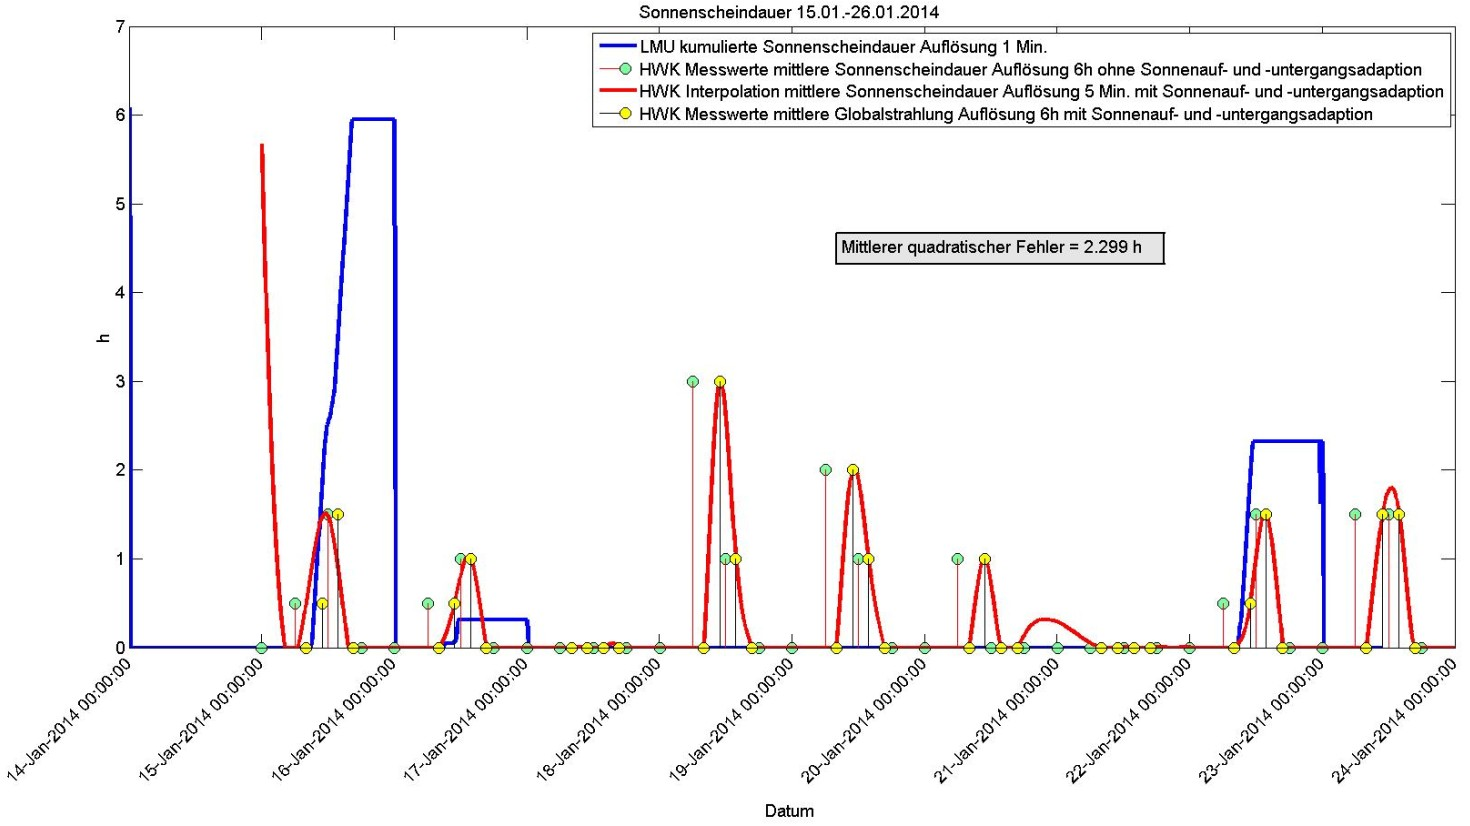
\includegraphics[width=16cm,height=10cm]{analyse/sonnensdauer2}
\caption{Vergleich der interpolierten Sonnenscheindauer mit den LMU Wetterdaten, Aufnahmetag 24.01.2014}
\label{fig:sonnensdauer}
\end{figure}
Bei der Sonnenscheindauer gibt es Diskrepanzen zwischen den Daten der LMU und denen der Wetterstation. Während die LMU keinen Sonnenschein ausweist, registriert die Wetterstation beispielsweise vom 18.01. bis einschließlich 20.01.2014 positive Werte. Dies kann an der Definition des Sonnenscheins liegen. In der Spezifikation der Station wird dann von Sonnenschein gesprochen, wenn die Globalstrahlung mehr als 120W/m² beträgt. Nach Rücksprache mit Herrn Lösslein von der LMU, wird bei den LMU Daten ebenfalls dieses Kriterium angewandt. Wie im Gespräch mit Herrn Volkhardt von der Firma HKW GmbH (Hersteller) zu ermitteln war, gibt es die Möglichkeit, solche Abweichungen beim Qualitätsmanagement des Wetterdienstes über die Firma HKW einzureichen \cite{TelHKW}. Da die Werte der LMU kumuliert sind, die der Wetterstation jedoch nicht, wird hier zum Vergleich der Prognosegüte nicht der RMSE verwendet. Es wird lediglich über die MATLAB Funktion \textsf{trapz} die Fläche unter den Spline-Kurven angenähert und dann mit dem maximalen Wert der LMU Daten verglichen. Hierbei fällt auf, dass die Prognose vom 22.01. näher an den realen Daten lag, als der dann tatsächlich vorliegende Wert der Wetterstation an diesem Tag. Für ein besseres Bild der Prognosegüte müssen mehr Daten ausgewertet werden.  
\begin{table}[t]
\caption{Absolute Abweichung der Sonnenscheindauer von den LMU Wetterdaten in Stunden}
\rowcolors{1}{cyan}{white}
{
\setlength{\extrarowheight}{0.1cm}
\begin{tabular}{| c | c | c | c | c | c | c | c | p{1cm} |}
\hline
\textbf{\parbox[t]{2.7cm}{Abrufdatum\\Intervall\\18.00-24.00 Uhr}} & \textbf{16.01.} & \textbf{17.01.} & \textbf{18.01.} & \textbf{19.01.} & \textbf{20.01.} & \textbf{21.01.} & \textbf{22.01.} & \textbf{23.01.} \\[1cm]
\hline \hline
\hiderowcolors
16.01.2014 & \cellcolor{red!25}2.66  & \cellcolor{green!25}0.11 &  &  &  &  &  & \\
17.01.2014 &  	    & \cellcolor{red!25}0.03 & \cellcolor{green!25}8.22 &  &  &  &  & \\
18.01.2014 &		& 		& \cellcolor{red!25}7.45 & \cellcolor{green!25}6.04 &  &  &  & \\
19.01.2014 &  	    &  	    & 	     & \cellcolor{red!25}5.49 & \cellcolor{green!25}2.54 &  &  &  \\ 
20.01.2014 &        &       &        &        & \cellcolor{red!25}2.18 & \cellcolor{green!25}0.08 &  & \\
21.01.2014 &        & 	    & 	     & 		  &  	   & \cellcolor{red!25}0.08 & \cellcolor{green!25}1.12 & \\
22.01.2014 &        & 	    & 	     & 		  &  	   & 						  & \cellcolor{red!25}1.83 & \cellcolor{green!25}4.21\\
\hline
\textbf{\parbox[t]{2.7cm}{prozentuale\\Abweichung\\der realen HKW Werte\\von der Prognose}}& & -73\% & -9,4\% & -9,1\% & -14,1\% & 0\% & +63\% & \\  
\hline
\end{tabular}
}
\label{tab:proggsd}
\end{table}
%Sonnenscheindauerende
\section{Globalstrahlung}
%Globalstrahlunganfang
Beim Vergleich der Globalstrahlung bietet sich ein geteiltes Bild. Im Bereich niedriger Globalstrahlung ($<$ 200W/m²) befindet sich der RMSE auf einem recht akzeptablen Niveau. Dies ändert sich jedoch bei großen Ausschlägen nach oben, wie sie am 22. und 23.01.2014 zu beobachten sind. Betrachtet man den 23.01. genauer, so lagen die Werte bei 75 und 100 W/m² für das Intervall von 6 Uhr bis 12 Uhr bzw. 12 bis 18 Uhr. Der Sonnenaufgang und der -untergang für diese Jahreszeit findet gegen 8 Uhr und 16.45 Uhr statt. D.h. ca. 250 W/m² fehlen dem eigentlich relevanten Intervall in dem die Sonne scheint. Verteilt man diese Energie auf die verbleibenden 9 Stunden, würde das die Kurve um ca. 28 W/m² nach oben verschieben. Die Daten der LMU erreichen an diesem Tag Spitzenwerte bis über 400 W/m². Die Werte fallen auch nicht nennenswert unter 100W/m², so dass davon ausgegangen werden kann, dass der mittlere Wert der LMU Daten höher liegt. Auch hier müsste man evtl. die Daten dem Anbieter der Wetterstation übergeben und vom Wetterdienst überprüfen lassen.   
\begin{figure}[htbp]
\centering
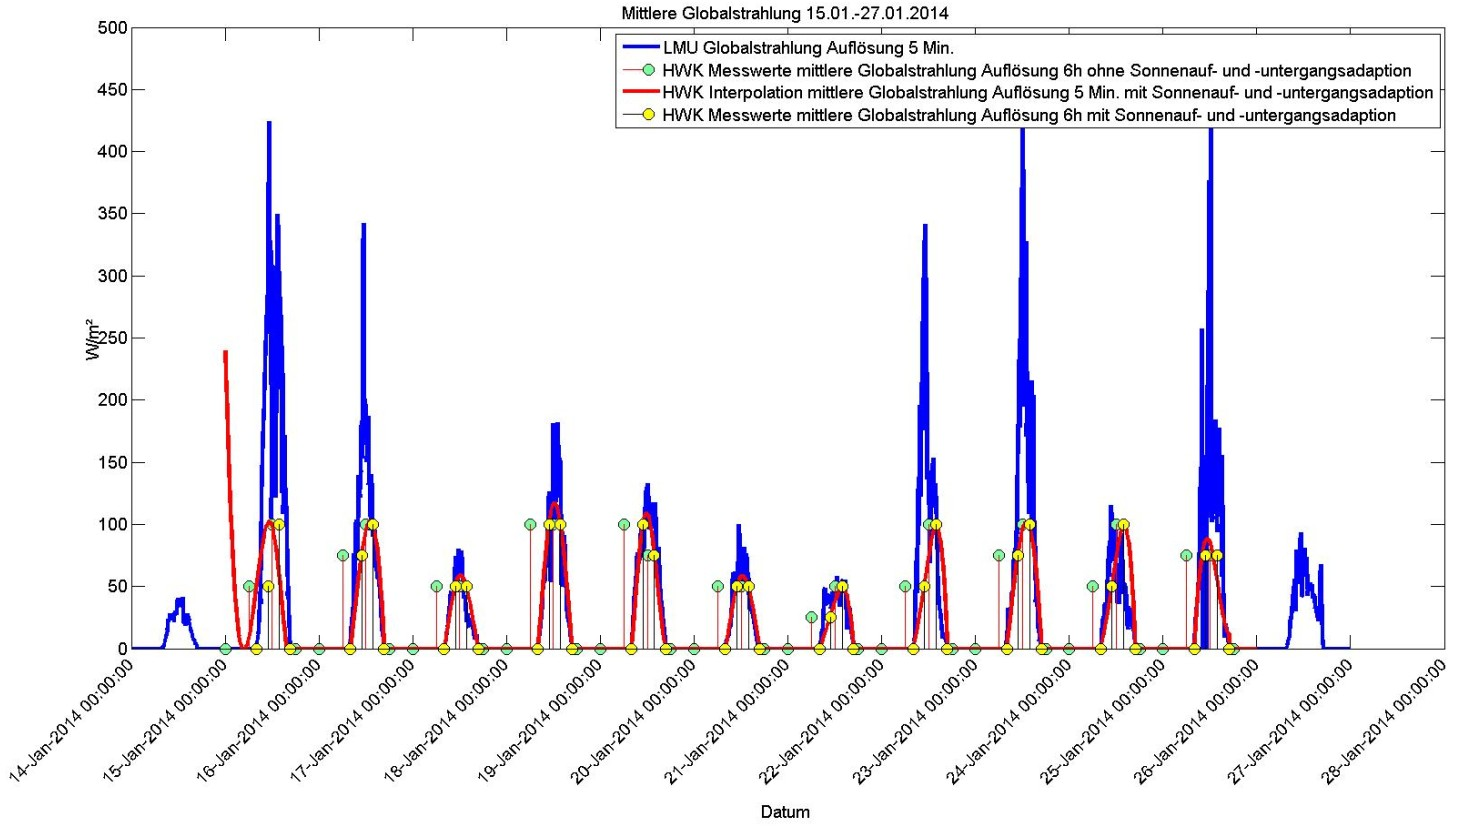
\includegraphics[width=16cm,height=10cm]{analyse/globalstr2}
\caption{Vergleich der interpolierten Globalstrahlung mit den LMU Wetterdaten, Aufnahmetag 24.01.2014}
\label{fig:globalstr}
\end{figure}
%Text
\begin{table}[t]
\caption{RMSE der Globalstrahlung in W/m²}
\rowcolors{1}{cyan}{white}
{
\setlength{\extrarowheight}{0.1cm}
\begin{tabular}{| c | c | c | c | c | c | c | c  | p{1.5cm} |}
\hline
\textbf{\parbox[t]{2.7cm}{Abrufdatum\\Intervall\\18.00-24.00 Uhr}} & \textbf{16.01.} & \textbf{17.01.} & \textbf{18.01.} & \textbf{19.01.} & \textbf{20.01.} & \textbf{21.01.} & \textbf{22.01.} & \textbf{23.01.} \\[1cm]
\hline \hline
\hiderowcolors
16.01.2014 & \cellcolor{red!25}38.11  & \cellcolor{green!25}5.10 &  &  &  &  &  & \\
17.01.2014 &  	   & \cellcolor{red!25}6.78 & \cellcolor{green!25}22.18 &  &  &  &  & \\
18.01.2014 &	   & 		& \cellcolor{red!25}16.37 & \cellcolor{green!25}13.22 &  &  &  & \\
19.01.2014 &  	   &  	    & 	     & \cellcolor{red!25}11.27 & \cellcolor{green!25}7.47 &  &  & \\ 
20.01.2014 &       &        &        &        & \cellcolor{red!25}7.36 & \cellcolor{green!25}12.09 &  & \\
21.01.2014 &       & 	    & 	     & 		  &  	   & \cellcolor{red!25}7.97 & \cellcolor{green!25}49.76 & \\
22.01.2014 &       & 	    & 	     & 		  &  	   & 						  & \cellcolor{red!25}59.81   & \cellcolor{green!25}68.55 \\
\hline
\textbf{\parbox[t]{2.7cm}{prozentuale\\Abweichung\\der realen HKW Werte\\von der Prognose}}& & +32.9\% & -26.2\% & -14.8\% & -1.5\% & -34.0\% & +20.2\% \\
\hline
\end{tabular}
}
\label{tab:proggsd}
\end{table}
%\begin{figure}[htbp]
%\centering
%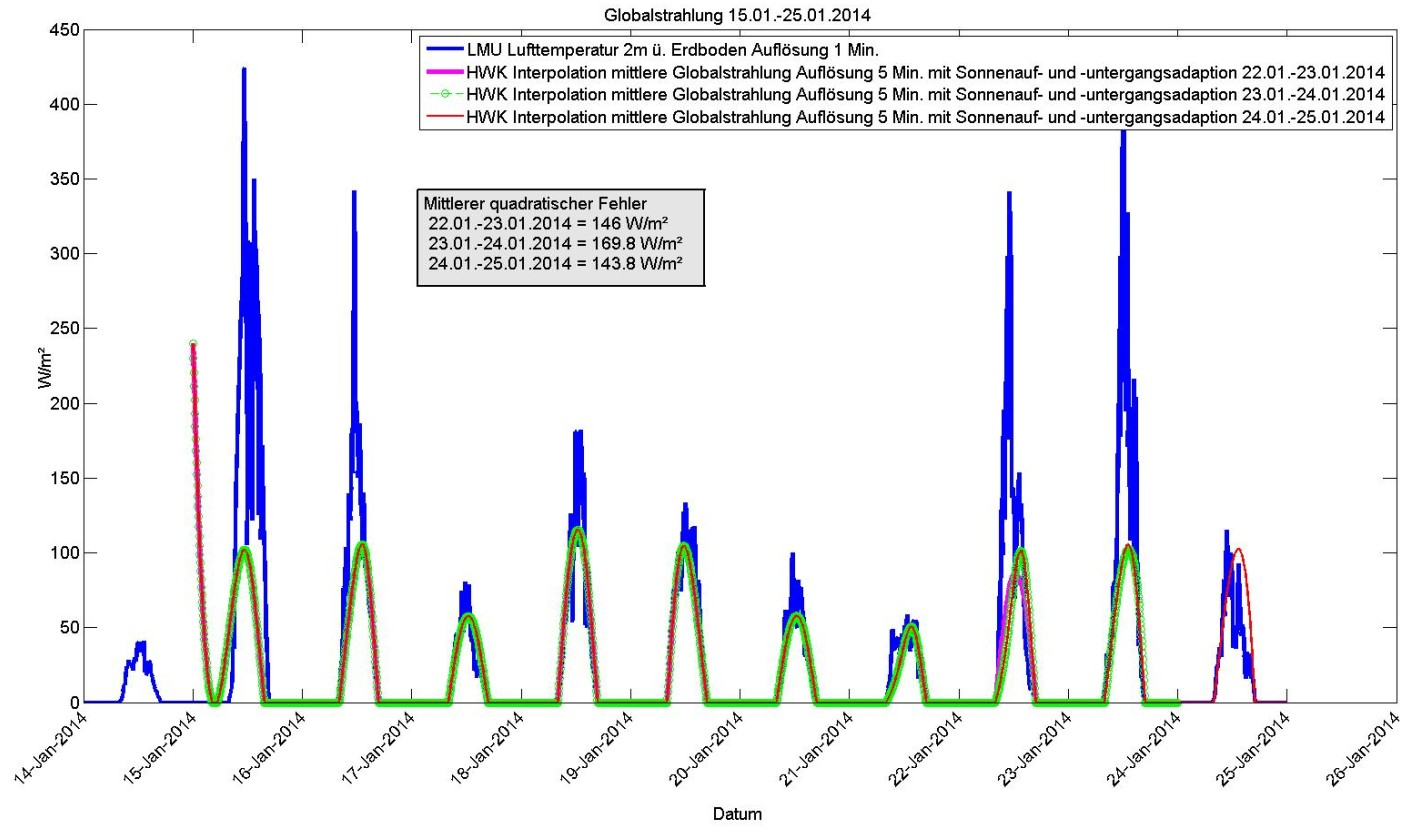
\includegraphics[width=16cm,height=10cm]{analyse/proggglob2}
%\caption{Prognosegüte für die Globalstrahlung}
%\label{fig:proggglob}
%\end{figure}
%Globalstrahlungende
\section{Niederschlagsmenge}
%Niederschlaganfang
Die Niederschlagsmenge wird ebenfalls wie zuvor schon die Solardaten mit einer 6 stündigen Auflösung bereit gestellt. Die Daten der LMU liegen in einer 1 Minuten Auflösung vor. Um die beiden Daten miteinander vergleichbar machen zu können, musste der HKW Wert mit einer Division durch 72 auf ein 5 Minuten Intervall gebracht werden. Im Gegensatz zur Globalstrahlung liegen hier die mittleren Werte der Wetterstation meist über denen der LMU. Betrachtet man den Prognoseverlauf vom 18.01. bis zum aktuellen Wert am 22.01. so erwartet man eine stetige Verbesserung der Werte, da weiter in der Zukunft liegende Prognosen unsicherer sind. Das ist aber nicht der Fall. Ob sich das auch über einen längeren Zeitraum hinzieht müsste mit einem größeren Datensatz überprüft werden. 
\begin{figure}[htbp]
\centering
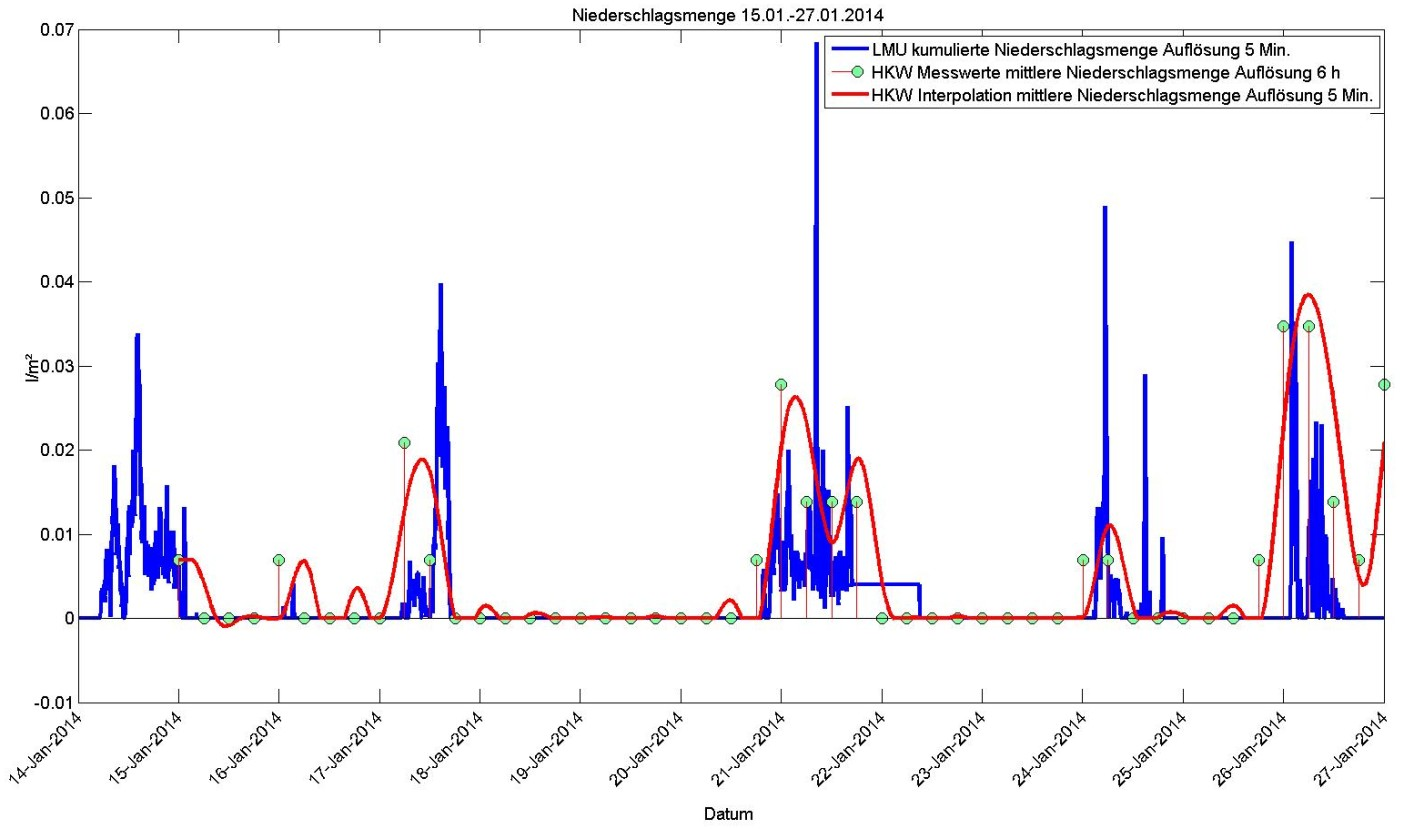
\includegraphics[width=16cm,height=10cm]{analyse/niedersmenge2}
\caption{Vergleich der interpolierten Niederschlagsmenge mit den LMU Wetterdaten, Aufnahmetag 24.01.2014}
\label{fig:niedersmenge}
\end{figure}
\begin{table}[t]
\caption{RMSE der Niederschlagsmenge in l/m²}
\rowcolors{1}{cyan}{white}
{
\setlength{\extrarowheight}{0.1cm}
\begin{tabular}{| c | p{1cm} | p{1cm} | p{1cm} | p{1cm} | p{1cm} | p{1cm} | p{1cm} | p{1cm} | p{1cm} |}
\hline
\textbf{\parbox[t]{2.3cm}{Abrufdatum\\Intervall\\18.00-24.00 Uhr}} & \textbf{16.01.} & \textbf{17.01.} & \textbf{18.01.} & \textbf{19.01.} & \textbf{20.01.} & \textbf{21.01.} & \textbf{22.01.} & \textbf{23.01.} & \textbf{24.01.} \\[1cm]
\hline \hline
\hiderowcolors
16.01.2014 & \cellcolor{red!25}0.22 & \cellcolor{green!25}0.43 & \cellcolor{yellow!25}0.04 & 0.00 &  &  &  &  & \\
17.01.2014 &  	    & \cellcolor{red!25}0.76 & \cellcolor{green!25}0.04 & \cellcolor{yellow!25}0.01 & 0.70 &  &  &  & \\
18.01.2014 &	    & 		& \cellcolor{red!25}0.04 & \cellcolor{green!25}0.03 & \cellcolor{yellow!25}0.82 & 1.14 &  &  & \\
19.01.2014 &  	    &  	    & 	     & \cellcolor{red!25}0.01 & \cellcolor{green!25}0.27 & \cellcolor{yellow!25}0.98 & 0.27 &  & \\ 
21.01.2014 &        &       &        &        & \cellcolor{red!25}0.38 & \cellcolor{green!25}1.40 & \cellcolor{yellow!25}0.07 & 0.23 & \\
22.01.2014 &        & 	    & 	     & 		  &  	   & \cellcolor{red!25}1.27 & \cellcolor{green!25}0.05 & \cellcolor{yellow!25}0.03 & 0.66 \\
\hline
\end{tabular}
}
\label{tab:proggns}
\end{table}
%Niederschlagende
\section{Windstärke}
%Windanfang
\begin{figure}[htbp]
\centering
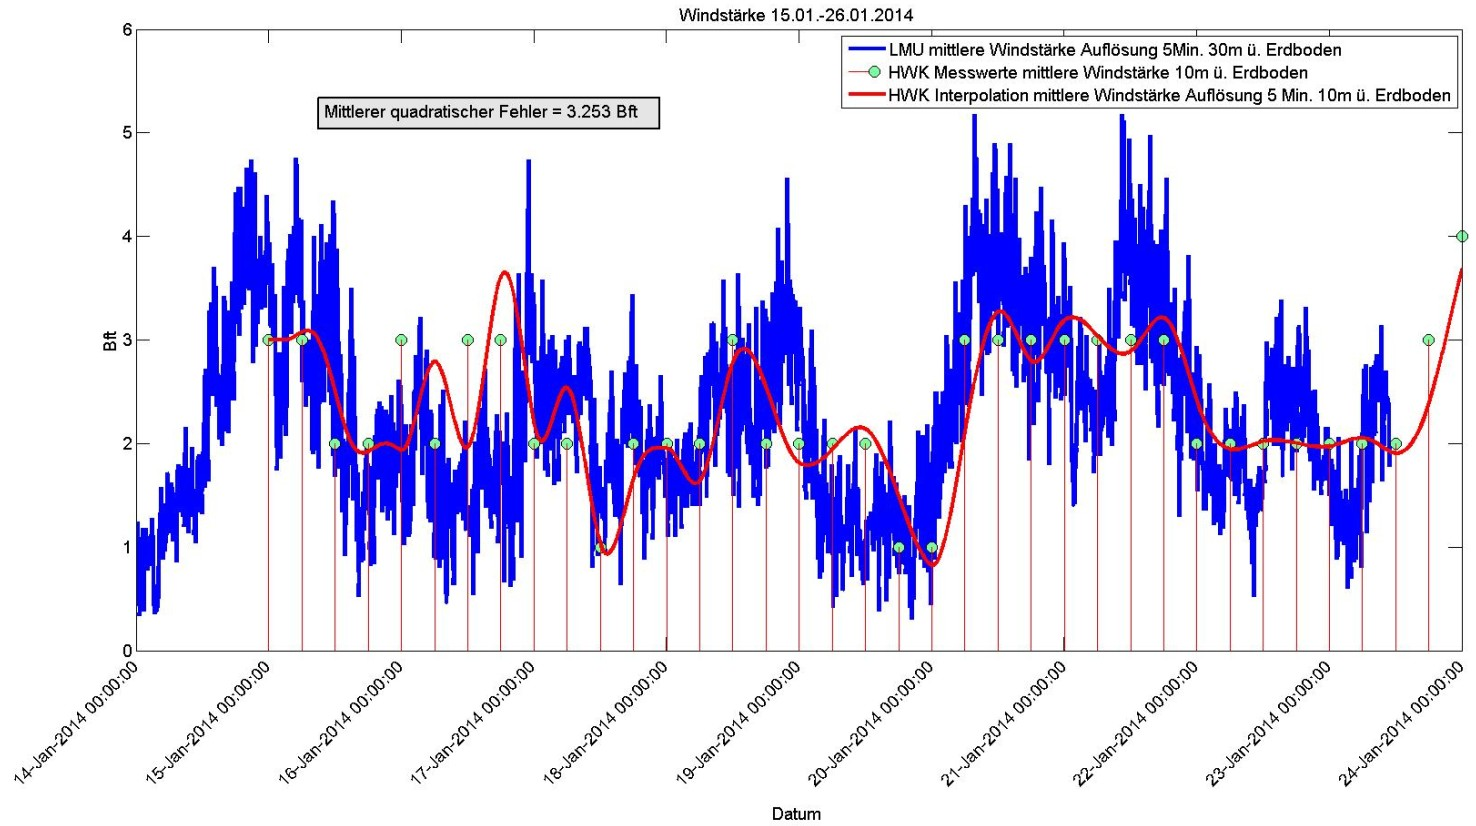
\includegraphics[width=16cm,height=10cm]{analyse/windstaerke2}
\caption{Vergleich der interpolierten Windstaerke mit den LMU Wetterdaten}
\label{fig:windstaerke}
\end{figure}
\begin{table}[t]
\caption{RMSE der Windstärke in Bft}
\rowcolors{1}{cyan}{white}
{
\setlength{\extrarowheight}{0.1cm}
\begin{tabular}{| c | p{1cm} | p{1cm} | p{1cm} | p{1cm} | p{1cm} | p{1cm} | p{1cm} | p{1cm} | p{1cm} |}
\hline
\textbf{\parbox[t]{2.3cm}{Abrufdatum\\Intervall\\18.00-24.00 Uhr}} & \textbf{16.01.} & \textbf{17.01.} & \textbf{18.01.} & \textbf{19.01.} & \textbf{20.01.} & \textbf{21.01.} & \textbf{22.01.} & \textbf{23.01.} & \textbf{24.01.} \\[1cm]
\hline \hline
\hiderowcolors
16.01.2014 & \cellcolor{red!25}1.23 & \cellcolor{green!25}0.66 & \cellcolor{yellow!25}0.81 & 0.76 &  &  &  &  & \\
17.01.2014 &  	   & \cellcolor{red!25}0.72 & \cellcolor{green!25}0.87 & \cellcolor{yellow!25}0.55 & 0.91 &  &  &  & \\
18.01.2014 &		   & 		& \cellcolor{red!25}0.78 & \cellcolor{green!25}0.72 & \cellcolor{yellow!25}1.32 & 0.91 &  &  & \\
19.01.2014 &  	   &  	    & 	     & \cellcolor{red!25}0.77 & \cellcolor{green!25}1.37 & \cellcolor{yellow!25}0.89 & 0.61 &  & \\ 
21.01.2014 &        &        &        &        & \cellcolor{red!25}1.07 & \cellcolor{green!25}0.91 & \cellcolor{yellow!25}0.65 & 0.94 & \\
22.01.2014 &        & 	    & 	     & 		  &  	   & \cellcolor{red!25}0.92 & \cellcolor{green!25}0.62 & \cellcolor{yellow!25}0.94 & 1.05 \\ 
\hline
\end{tabular}
}
\label{tab:proggwind}
\end{table}
 
Die Windstärkedaten der LMU sind mit einer Auflösung von einer Minute äußerst genau, was sich in den häufigen Ausschlägen widerspiegelt. Dennoch folgt der Graph der interpolierten Daten relativ gut dem Gesamtverlauf. Da die Windstärke in einer Höhe von 30m an der LMU gemessen wird, lassen sich evtl. die Abweichungen von einem Bft erklären. Die Daten der Wetterstation beziehen sich auf 10m über dem Erdboden. 

Geht man zum Beispiel von einer Stärke von 3 Bft auf 10m Höhe aus, dann kann man über das logarithmische Grenzschichtprofil die Windstärke in 30m Höhe abschätzen. Die Formel hierzu lautet: \(v(30m) = v(10m)*\frac{ln(\frac{30m-0}{2})}{ln(\frac{10m-0}{2})}\). Mit einer Geländeklasse, die einem Stadtkern entspricht, ergibt sich bei einer Geschwindigkeit von 4,4m/s für v(10m) und keinem Versatz der Grenzschicht durch Hindernisse ein Wert von 7,4m/s, der ungefähr einem Bft mehr entspricht \cite{GrenzProf}.

Wie gut nun die Prognosewerte sind, darüber lässt sich eine Aussage mit dem Root Mean Squared Error (RMSE) treffen \cite{DWD}. Dieser stellt die Standardabweichung der Differenzen zwischen Prognose- und Beobachtungswert dar. Der Deutsche Wetterdienst empfiehlt in seiner Broschüre keine größere Abweichung als 1 Bft für eine gute Prognose. Die nachfolgende Tabelle stellt jeweils den RMSE für unterschiedliche Abrufdaten dar. Dabei steht der rot markierte Bereich für den aktuellen Tag, der Grüne für den ersten Folgetag, der Gelbe für den zweiten Folgetag und der Weiße für den dritten Folgetag. Wie man in der Tabelle \ref{tab:proggwind} erkennen kann, wird dieses Qualitätsmerkmal weitgehend eingehalten. 
%Windende 
\section{Mittlere Lufttemperatur}
%Luftanfang 
Die mittlere Lufttemperatur wird mit einer 1 stündigen Auflösung an die Wetterstation übertragen. Es ist deshalb davon auszugehen, dass diese Daten verglichen mit den Daten der LMU weniger große Diskrepanzen aufweisen. Betrachtet man die Abbildung \ref{fig:mittlufttemp} so vermittelt diese, einen die vorige Aussage bestätigenden Eindruck. Auffallend jedoch ist der teilweise Versatz der Datenpunkte nach unten. Ein Blick auf den RMSE in der Tabelle \ref{tab:progglufttemp} zeigt, dass es sich hierbei meist um 1 bis 2 $^\circ$C bei den tagesaktuellen Daten und 1 bis 3,5 $^\circ$C bei den Prognosedaten handelt. Ein Grund für diese eher einseitige Abweichung nach unten könnte ein unterschiedlicher Standort der beiden Wetterstationen sein. Die LMU Wetterstation befindet sich direkt im Stadtzentrum. Bewegt man sich hin zu den Randbezirken Münchens, kann die Temperatur um bis zu 6 $^\circ$C abfallen \cite{stadtklima}. Auch hier ist der Verlauf der Prognoseentwicklung nicht immer der, den man erwarten würde. Nimmt man zum Beispiel den 19. Januar so war die Prognose am 16.01.2014 für diesen Tag besser als die beiden Darauffolgenden, die weniger weit in die Zukunft reichen. Hinsichtlich der Prognosegüte kann man unter Berücksichtigung des vermutlichen Standortunterschieds gem. dem DWD von einer guten Vorhersage ausgehen. Dieser gibt hierfür einen Grenzwert von 2,5 $^\circ$C (RMSE) vor \cite{DWD}. Um diesen evtl. standortabhängigen Temperatureffekt zu korrigieren, bietet es sich vielleicht an, den in der Wetterstation integrierten Temperatursensor mitzuverwenden. Eine historische Auswertung der Daten und ein daraus ermittelter Korrekturfaktor könnten den Offset ausgleichen.        
\begin{figure}[h]
\centering
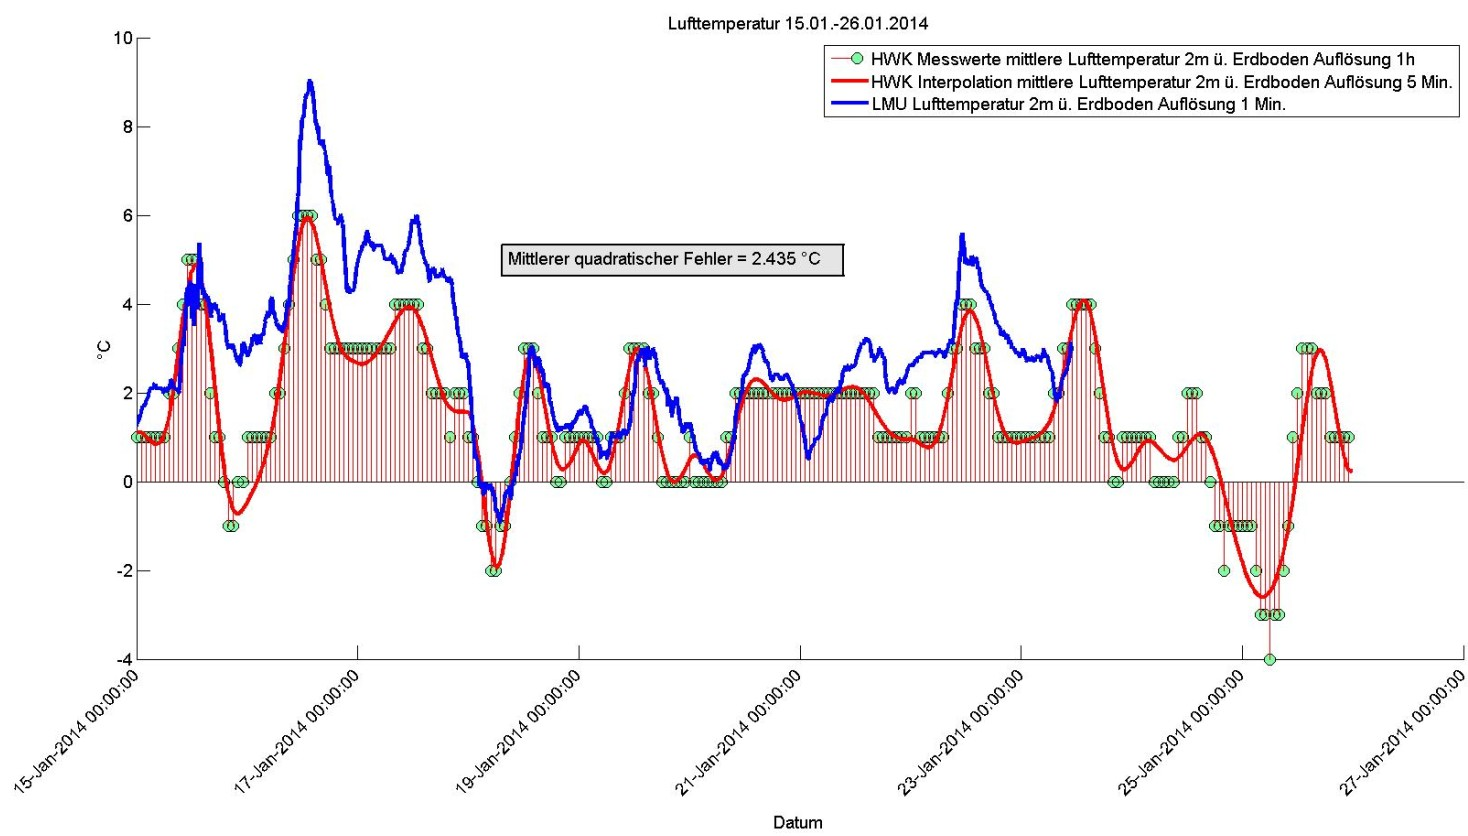
\includegraphics[width=16cm,height=10cm]{analyse/mittlufttemp2}
\caption{Vergleich der interpolierten mittleren Lufttemperatur mit den LMU Wetterdaten, Aufnahmetag 24.01.2014}
\label{fig:mittlufttemp}
\end{figure}
\begin{table}[h]
\caption{RMSE der mittleren Lufttemperatur in $^\circ$C}
\rowcolors{1}{cyan}{white}
{
\setlength{\extrarowheight}{0.1cm}
\begin{tabular}{| c | p{1cm} | p{1cm} | p{1cm} | p{1cm} | p{1cm} | p{1cm} | p{1cm} | p{1cm} | p{1cm} |}
\hline
\textbf{\parbox[t]{2.7cm}{Abrufdatum\\Intervall\\18.00-24.00 Uhr}} & \textbf{16.01.} & \textbf{17.01.} & \textbf{18.01.} & \textbf{19.01.} & \textbf{20.01.} & \textbf{21.01.} & \textbf{22.01.} & \textbf{23.01.} & \textbf{24.01.} \\[1cm]
\hline \hline
\hiderowcolors
16.01.2014 & \cellcolor{red!25}2.30 & \cellcolor{green!25}2.65 & \cellcolor{yellow!25}2.03 & 1.35 &  &  &  &  & \\
17.01.2014 &  	   & \cellcolor{red!25}2.04 & \cellcolor{green!25}2.81 & \cellcolor{yellow!25}1.90 & 0.77 &  &  &  & \\
18.01.2014 &		   & 		& \cellcolor{red!25}0.81 & \cellcolor{green!25}2.07 & \cellcolor{yellow!25}1.13 & 1.08 &  &  & \\
19.01.2014 &  	   &  	    & 	     & \cellcolor{red!25}0.99 & \cellcolor{green!25}0.58 & \cellcolor{yellow!25}0.61 & 2.84 &  & \\ 
20.01.2014 &        &        &        &        & \cellcolor{red!25}0.53 & \cellcolor{green!25}1.08 & \cellcolor{yellow!25}3.21 & 3.66 & \\
21.01.2014 &        & 	    & 	     & 		  &  	   & \cellcolor{red!25}1.03 & \cellcolor{green!25}3.01 & \cellcolor{yellow!25}2.77 & 2.76 \\
\hline
\end{tabular}
}
\label{tab:progglufttemp}
\end{table}
%Luftende